\documentclass[a4paper, twoside, english]{article}

\usepackage{amsmath}
\usepackage{amsfonts}
\usepackage{ihci}
\usepackage{graphicx}
\usepackage{subfig}
\usepackage{listings}
\usepackage{color}

% Unicode workaround for lstlistings
\lstset{literate=
	{á}{{\'a}}1 {é}{{\'e}}1 {í}{{\'i}}1 {ó}{{\'o}}1 {ú}{{\'u}}1
	{Á}{{\'A}}1 {É}{{\'E}}1 {Í}{{\'I}}1 {Ó}{{\'O}}1 {Ú}{{\'U}}1
	{à}{{\`a}}1 {è}{{\`e}}1 {ì}{{\`i}}1 {ò}{{\`o}}1 {ù}{{\`u}}1
	{À}{{\`A}}1 {È}{{\'E}}1 {Ì}{{\`I}}1 {Ò}{{\`O}}1 {Ù}{{\`U}}1
	{ä}{{\"a}}1 {ë}{{\"e}}1 {ï}{{\"i}}1 {ö}{{\"o}}1 {ü}{{\"u}}1
	{Ä}{{\"A}}1 {Ë}{{\"E}}1 {Ï}{{\"I}}1 {Ö}{{\"O}}1 {Ü}{{\"U}}1
	{â}{{\^a}}1 {ê}{{\^e}}1 {î}{{\^i}}1 {ô}{{\^o}}1 {û}{{\^u}}1
	{Â}{{\^A}}1 {Ê}{{\^E}}1 {Î}{{\^I}}1 {Ô}{{\^O}}1 {Û}{{\^U}}1
	{œ}{{\oe}}1 {Œ}{{\OE}}1 {æ}{{\ae}}1 {Æ}{{\AE}}1 {ß}{{\ss}}1
	{ű}{{\H{u}}}1 {Ű}{{\H{U}}}1 {ő}{{\H{o}}}1 {Ő}{{\H{O}}}1
	{ç}{{\c c}}1 {Ç}{{\c C}}1 {ø}{{\o}}1 {å}{{\r a}}1 {Å}{{\r A}}1
	{€}{{\euro}}1 {£}{{\pounds}}1 {«}{{\guillemotleft}}1
	{»}{{\guillemotright}}1 {ñ}{{\~n}}1 {Ñ}{{\~N}}1 {¿}{{?`}}1
}

% Define Synatx highlighting for Python
\definecolor{maroon}{cmyk}{0, 0.87, 0.68, 0.32}
\definecolor{halfgray}{gray}{0.55}
\definecolor{ipython_frame}{RGB}{207, 207, 207}
\definecolor{ipython_bg}{RGB}{247, 247, 247}
\definecolor{ipython_red}{RGB}{186, 33, 33}
\definecolor{ipython_green}{RGB}{0, 128, 0}
\definecolor{ipython_cyan}{RGB}{64, 128, 128}
\definecolor{ipython_purple}{RGB}{170, 34, 255}

\lstdefinelanguage{iPython}{
	morekeywords=[1]{access,and,break,class,continue,def,del,elif,else,except,exec,finally,for,from,global,if,import,in,is,lambda,not,or,pass,print,raise,return,try,while},%
	%
	% Built-ins
	morekeywords=[2]{abs,all,any,basestring,bin,bool,bytearray,callable,chr,classmethod,cmp,compile,complex,delattr,dict,dir,divmod,enumerate,eval,execfile,file,filter,float,format,frozenset,getattr,globals,hasattr,hash,help,hex,id,input,int,isinstance,issubclass,iter,len,list,locals,long,map,max,memoryview,min,next,object,oct,open,ord,pow,property,range,raw_input,reduce,reload,repr,reversed,round,set,setattr,slice,sorted,staticmethod,str,sum,super,tuple,type,unichr,unicode,vars,xrange,zip,apply,buffer,coerce,intern},%
	%
	sensitive=true,%
	morecomment=[l]\#,%
	morestring=[b]',%
	morestring=[b]",%
	%
	morestring=[s]{'''}{'''},% used for documentation text (mulitiline strings)
	morestring=[s]{"""}{"""},% added by Philipp Matthias Hahn
	%
	morestring=[s]{r'}{'},% `raw' strings
	morestring=[s]{r"}{"},%
	morestring=[s]{r'''}{'''},%
	morestring=[s]{r"""}{"""},%
	morestring=[s]{u'}{'},% unicode strings
	morestring=[s]{u"}{"},%
	morestring=[s]{u'''}{'''},%
	morestring=[s]{u"""}{"""},%
	morestring=[s]{f'}{'},% format strings
	morestring=[s]{f"}{"},%
	morestring=[s]{f'''}{'''},%
	morestring=[s]{f"""}{"""},%
	%
	identifierstyle=\color{black}\ttfamily,
	commentstyle=\color{ipython_cyan}\ttfamily,
	stringstyle=\color{ipython_red}\ttfamily,
	keepspaces=true,
	showspaces=false,
	showstringspaces=false,
	%
	rulecolor=\color{ipython_frame},
	frame=single,
	frameround={t}{t}{t}{t},
	framexleftmargin=6mm,
	numbers=left,
	numberstyle=\tiny\color{halfgray},
	%
	%
	backgroundcolor=\color{ipython_bg},
	extendedchars=true,
	basicstyle={\small\ttfamily},
	keywordstyle=[1]{\color{ipython_green}\ttfamily},
	keywordstyle=[2]{\color{ipython_purple}\ttfamily},
}

\graphicspath{{./../figures/}}

\title{Machine Learning Project\\Task 1 Report}  % Replace "Template Report" with Exercise 1, Exercise 2, etc
\author{Albert Garaev, Ksenia Novikova, Mukhammadsodik Khabibulloev }    % Replace with your names
\date{27.11.2021}                              % Replace with current date

\begin{document}

\maketitle


\section{K Nearest Neighbour Classification}
\subsection{Tasks}

\begin{figure}[h!]
	\centerline{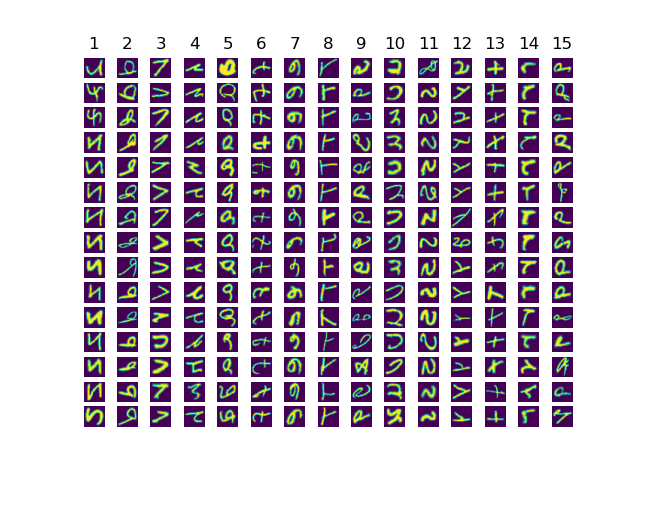
\includegraphics[width=0.95\textwidth]{all_classes.png}}
	\caption[classes]{Examples of all classes}
	\label{fig:classes_ex}
\end{figure}

The Figure\ref{fig:classes_ex} shows the plot of 15 random images from each of 15 classes. From plotted data, we can assume that the dataset contains 15 letters of the alphabet in their handwritten form.\\


For this dataset we implemented KNN algorithm with 5-fold cross validation and different distance measures. The source code of cross validation function is shown below.\\

\newpage
\begin{lstlisting}[language=iPython]
def cross_validation(X, Y, Xtest, Ytest, m=5):
	trainX = X
	trainY = Y
	kn = KNN()
	neighb = [1, 2, 3, 4, 5, 6, 7, 8, 9, 10]
	trainX_fold = np.array_split(trainX, m)
	trainY_fold = np.array_split(trainY, m)
	k_to_acc = {}
	for k in neighb:
		k_to_acc[k] = list()
	for k in neighb:
		print('k=', k)
	for i in range(m):
		X_val = trainX_fold[i]
		Y_val = trainY_fold[i]
		X_tr = np.vstack((trainX_fold[0:i] + trainX_fold[i + 1:]))
		Y_tr = np.vstack((trainY_fold[0:i] + trainY_fold[i + 1:])).ravel()
		knnf = KNN()
		knnf.fit(X_tr, Y_tr)
		pred = knnf.predict(X_val, k=k)
		acc = np.mean(pred == Y_val)
		k_to_acc[k].append(acc)
	scores = []
	best_k = 0
	best_acc = 0
	for k in neighb:
		acc = np.mean(k_to_acc[k])
		print(acc)
		scores.append(acc)
		if acc > best_acc:
			best_acc = acc
			best_k = k
	clf = KNN()
	clf.fit(trainX, trainY)
	y_test_pred = clf.predict(Xtest, k=best_k)
	acc = np.mean(y_test_pred == Ytest)
	print('Acc:{}, best_k:{}'.format(acc, best_k))			
\end{lstlisting}
Except the Euclidean distance, we also used Manhattan distance metric to measure distance between vectors and to evaluate our algorithm. According to this Manhattan distance, the distance between two points is equal to the sum of the absolute values of the differences of their coordinates.\\

This code shows functions for distance metrics. \\

\begin{lstlisting}[language=iPython]
	def euclidean_distance(a, b):
	return np.sqrt(np.sum(np.square(a - b), axis=1))
	
	def manhattan_distance(a, b):
	return np.abs(np.array(a) - np.array(b)).sum(axis=1)
	
	def haming_distance(a, b):
	return sum(el1 != el2 for el1, el2 in zip(a, b))
\end{lstlisting}

\newpage
Using euclidean distance, we got best accuracy with k=4. The plot of dependence of accuracy on k is shown in Figure ~\ref{fig:Euclid_dist}.\\

\begin{figure}[h!]
	\centerline{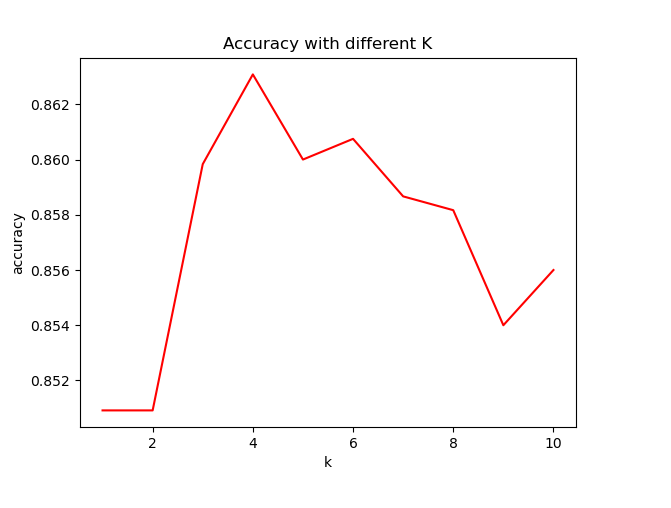
\includegraphics[width=0.6\textwidth]{euc_plot.png}}
	\caption[classes]{Accuracy with different k (Euclidean distance)}
	\label{fig:Euclid_dist}
\end{figure}

Using manhattan distance, we got best accuracy with k=6. The plot of dependence of accuracy on k is shown in Figure \ref{fig:Manh_dist}.\\

\begin{figure}[h!]
	\centerline{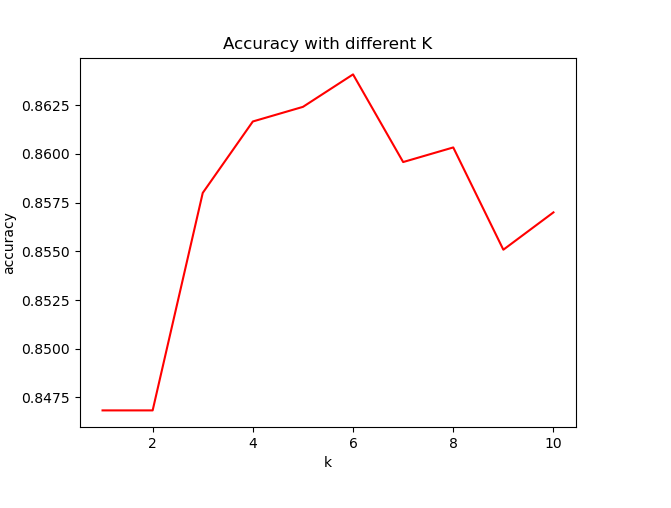
\includegraphics[width=0.6\textwidth]{manh_plot.png}}
	\caption[classes]{Accuracy with different k (Manhattan distance)}
	\label{fig:Manh_dist}
\end{figure}

\newpage
 
At the next step we implemented convolutional operation and applied filters to images. The first filter blures images and the second is edge detection filter. The code of convolutional function is shown bellow.\\

\begin{lstlisting}[language=iPython]
def convolve2D(image, kernel, padding=0, strides=1):
    kernel = np.flipud(np.fliplr(kernel))
    xKernShape = kernel.shape[0]
    yKernShape = kernel.shape[1]
    xImgShape = image.shape[0]
    yImgShape = image.shape[1]

    xOutput = int(((xImgShape - xKernShape + 2 * padding) / strides) - 1)
    yOutput = int(((yImgShape - yKernShape + 2 * padding) / strides) - 1)
    output = np.zeros((xOutput, yOutput))

    if padding != 0:
        imagePadded = np.zeros((image.shape[0] + padding*2, image.shape[1]
 + padding*2))
        imagePadded[int(padding):int(-1 * padding), int(padding):int(-1 * padding)] = image
        print(imagePadded)
    else:
        imagePadded = image

    for y in range(image.shape[1]):
        # Exit Convolution
        if y > image.shape[1] - yKernShape:
            break
        if y % strides == 0:
            for x in range(image.shape[0]):
                if x > image.shape[0] - xKernShape:
                    break
                try:
                    if x % strides == 0:
                        output[x, y] =
 (kernel * imagePadded[x: x + xKernShape, y: y + yKernShape]).sum()
                except:
                    break
    return output
\end{lstlisting}

\newpage
Figure \ref{fig:blur} shows images of dataset after bluring.

\begin{figure}[h!]
	\centerline{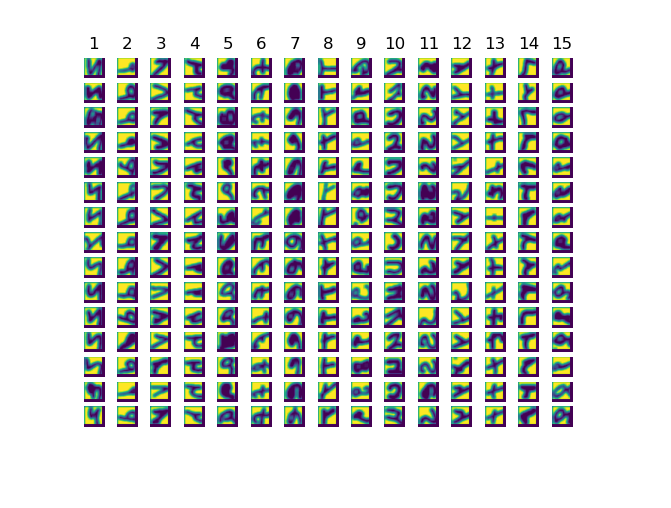
\includegraphics[width=0.8\textwidth]{blured_data.png}}
	\caption[classes]{Images with blur filter}
	\label{fig:blur}
\end{figure}


Figure \ref{fig:edge} shows images after edge detection filter.


\begin{figure}[h!]
	\centerline{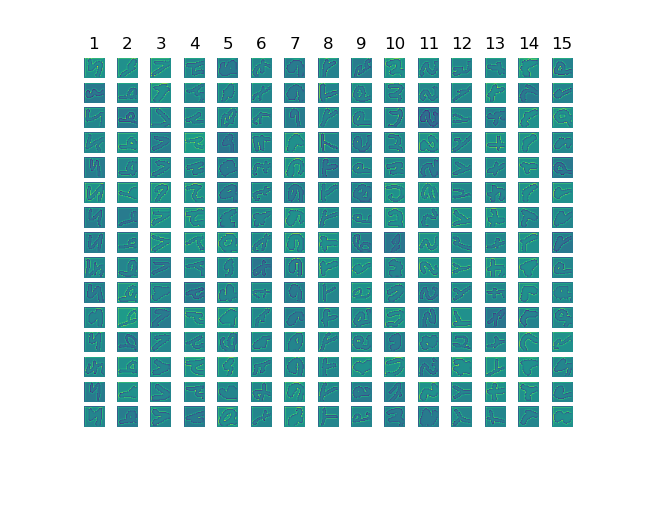
\includegraphics[width=0.8\textwidth]{edge_data.png}}
	\caption[classes]{Images with edge detection filter}
	\label{fig:edge}
\end{figure}
\newpage

We applied knn algorithm with 5-fold cross validation on filtered images. Figures 6 and 7 shows results of accuracy measuring.  On images with edge detection filter we got accuracy less than 50. The plots of dependence of accuracy on k are shown at Figure \ref{fig:acc_blur} and Figure \ref{fig:acc_edge}.\\

\begin{figure}[h!]
	\centerline{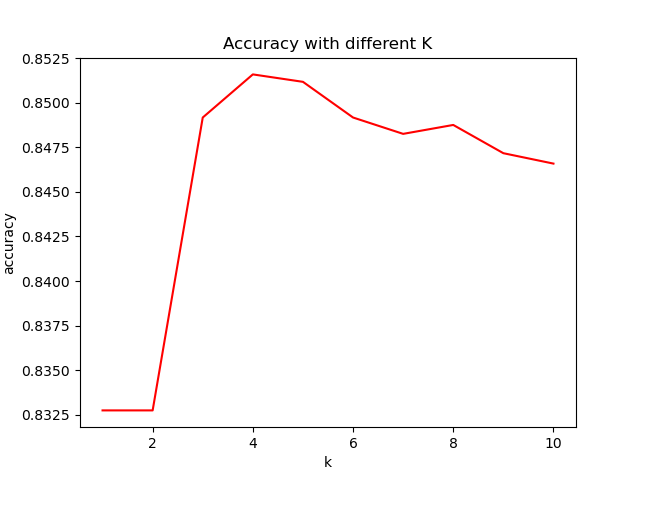
\includegraphics[width=0.8\textwidth]{blured_accuracy.png}}
	\caption[classes]{Accuracy with different k (Blured images)}
	\label{fig:acc_blur}
\end{figure}

\begin{figure}[h!]
	\centerline{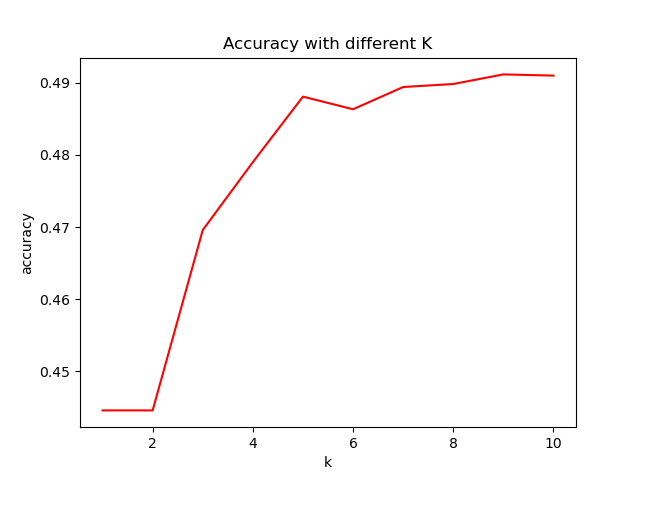
\includegraphics[width=0.8\textwidth]{edge_accuracy.png}}
	\caption[classes]{Accuracy with different k (Images with edge detection)}
	\label{fig:acc_edge}
\end{figure}
\newpage
Next, we used extended version of kNN algorithm with weighted kNN. Using euclidean distance metrics with weighted kNN we got the best accuracy with k=6. The plot of dependence of accuracy on k is shown in Figure \ref{fig:acc_KNN}.\\

\begin{figure}[h!]
	\centerline{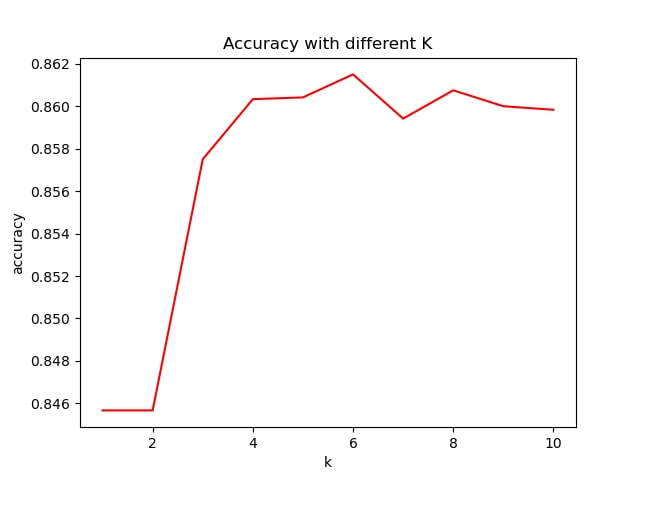
\includegraphics[width=0.9\textwidth]{weight.png}}
	\caption[classes]{Accuracy on weighted kNN}
	\label{fig:acc_KNN}
\end{figure}




\newpage
\section{Deep Neural Networks}
\subsection{Tasks}
\textit{Activation function}. In artificial neural networks, the neuron activation function determines the output signal, which is determined by the input signal or a set of input signals. For instance, using activation function Rectified linear unit (ReLU), if the input value is less than 0, then this function equates to zero, otherwise the value remains the same.\\

\textit{Loss function}. The loss function is used to calculate the error between real and received responses. Our global goal is to minimize this error. Thus, the loss function brings neural network training closer to this goal. An example of a loss function is cross-entropy, which describes the distance between the actual outcome (probability) and the expected outcome (probability), that is, the smaller the cross-entropy value, the closer the two probability distributions.\\

\textit{Hyperparameters} is a manually configurable parameter used to regulate network learning. For instance, a model hyperparameter is size of a neural network and its topology.\\ 

\textit{Optimizers} determine the optimal set of model parameters, such as weight, so that the model produces the best results when solving a specific problem. Examples of optimizers: SGD, Adam, Adagrad, Adamax.\\ 

\textit{Epoch}. One epoch has occurred, which means the entire dataset has passed through the neural network in the forward and backward directions only once. With an increase in the number of epochs, the weights of the neural network change more and more times. One epoch leads to underfitting, and an excess of epochs leads to overfitting.\\ 

\textit{Underfitting} might occur when using insufficiently complex models. The training algorithm does not provide a sufficiently small value of the average error on the training sample.\\

\textit{Overfitting}. The model explains well only examples from the training set, adapting to training examples, instead of learning to classify examples that were not involved in training (losing the ability to generalize).\\

\textit{Training set} is a sequence of data that a neural network uses. It contains examples with true values like tags, classes, metrics. Unlabeled sets are also used to train neural networks.\\

\textit{Test set} is used for estimation of the generalization error of the model which we choose. The test set should be used only at the end of the data analysis.\\

\textit{Validation set} is used for estimation of prediction error, in this regard we can choose optimal model. The division into sets can be carried out approximately in the following proportions: training set 60\%, test set 20\%, validation set 20\%. Sometimes there is no validation set, in this case we can divide data like training set 70\%, test set 30\%.\\
\newpage

\textit{Training network on the Strange Symbols dataset.}\\

Number of epochs and the training loss are shown in Figure \ref{fig:loss}\\
\begin{figure}[h!]
	\centerline{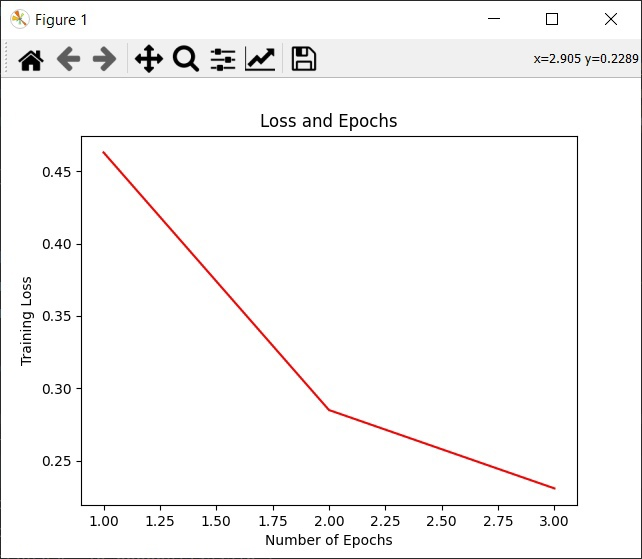
\includegraphics[width=0.55\textwidth]{loss.png}}
	\caption[loss]{Number of epochs and the training loss}
	\label{fig:loss}
\end{figure}
Number of epochs and the accuracy are shown in Figure \ref{fig:acc}\\
\begin{figure}[h!]
	\centerline{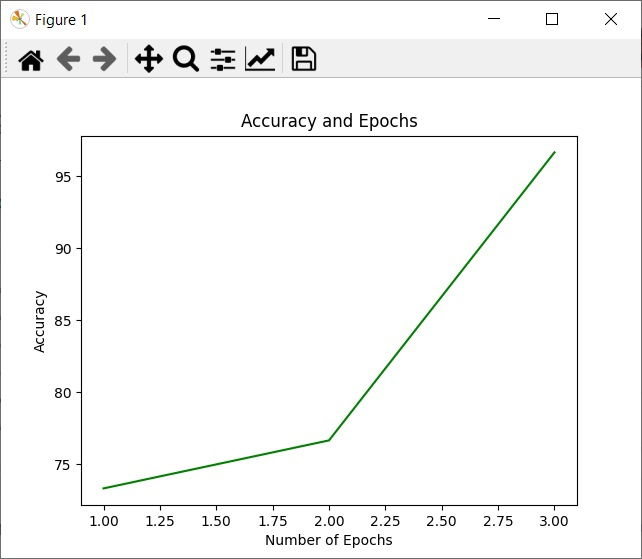
\includegraphics[width=0.55\textwidth]{acc.png}}
	\caption[acc]{Number of epochs and the accuracy}
	\label{fig:acc}
\end{figure}
\newpage
Description of our best architecture of network.\\
\begin{lstlisting}[language=iPython]
	class Net(nn.Module):
	def __init__(self):
	super(Net, self).__init__()
	
	# Declaration of  the layers for feature extraction
	self.features = nn.Sequential(nn.Conv2d(
	in_channels=1, #Number of channels in the input image
	out_channels=10, #Number of channels produced by the convolution
	kernel_size=3, #Size of the convolving kernel
	stride=1,
	padding=1),
	nn.ReLU(inplace=True),
	nn.Conv2d(
	in_channels=10,
	out_channels=30,
	kernel_size=3,
	stride=1,
	padding=1),
	nn.MaxPool2d(2, 2),
	nn.ReLU(inplace=True),
	nn.BatchNorm2d(30),
	nn.Conv2d(
	in_channels=30,
	out_channels=90,
	kernel_size=3,
	stride=1,
	padding=1),
	nn.ReLU(inplace=True),
	nn.BatchNorm2d(90)) #90 number of channels from input
	
	# Layers for classification
	# In feature extraction layers, 1 max merge layer, which halves the
	# height and width of the image, so we get a size of 14 x 14 (28/2)
	# with the last output out_channels 90.
	# We transfer them to a sequential layer.
	# Here we used hidden layers of 512 and 256 neurons.
	self.classifier = nn.Sequential(
	nn.Linear(14 * 14 * 90, 512),
	nn.ReLU(inplace=True),
	nn.Dropout(0.5), # input randomly zeroes with probability p=0.5
	nn.Linear(512, 256),
	nn.ReLU(inplace=True),
	nn.Linear(256, 15)) #Output layer 15 (number of classes)
	
\end{lstlisting}

\newpage
The confusion matrix is shown in Figure \ref{fig:matr}. The output will be a series of 15 (number of classes) lists. The diagonal values from top to bottom from left to right is the number of correctly predicted values for each class.\\
\begin{figure}[h!]
	\centerline{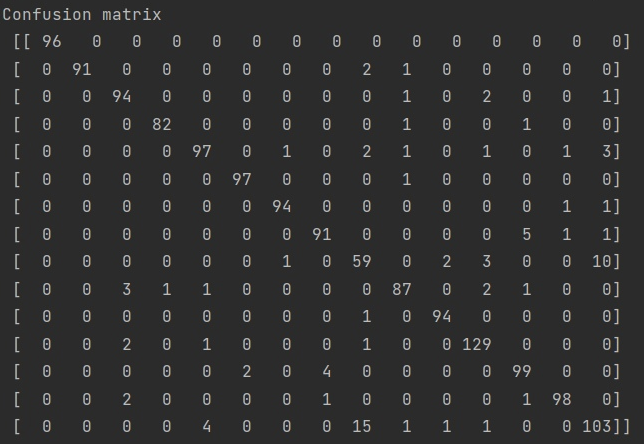
\includegraphics[width=0.55\textwidth]{conf_matrix.png}}
	\caption[matrix]{Confusion matrix}
	\label{fig:matr}
\end{figure}


As we can see at the confusion matrix the worst result (59) of recognition show the class 8. We can see how images of this class looks like in Figure~\ref{fig:cl8}.\\
\begin{figure}[h!]
	\centerline{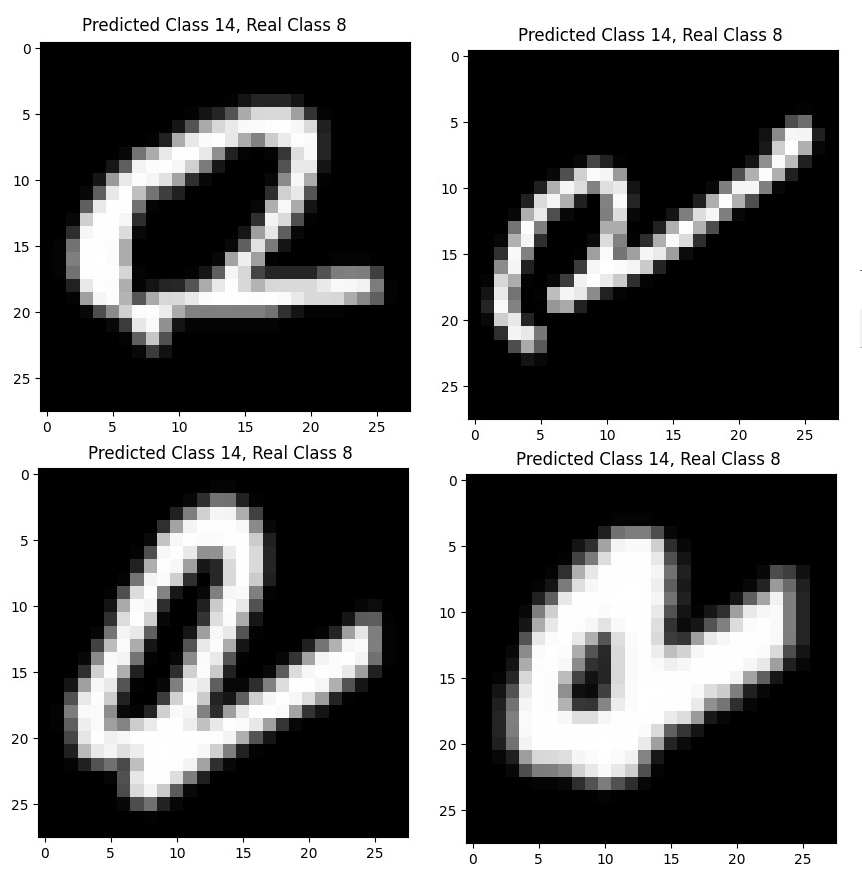
\includegraphics[width=0.35\textwidth]{class8_bad.png}}
	\caption[cl8]{Predictions for class 8}
	\label{fig:cl8}
\end{figure}
\newpage

We can see that model predict for class 8 that it is class 14. We can see how images of class 14 looks in  Figure~\ref{fig:cl14}.\\

\begin{figure}[hb]
	\centerline{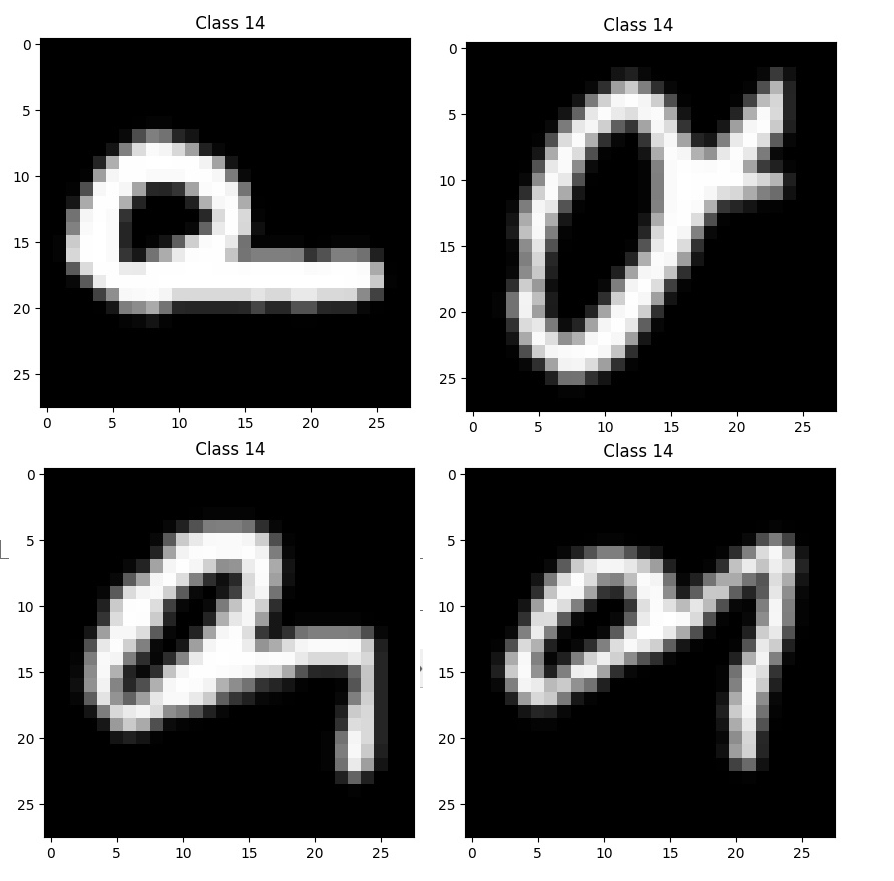
\includegraphics[width=0.35\textwidth]{class14_w8.png}}
	\caption[cl14]{Images of class 14}
	\label{fig:cl14}
\end{figure}

We can see that the images of classes 8 and 14 looks almost the same, this fact affects the accuracy of predictions.\\
Now we see the well predicted classes, for instance, class 11 and class 6 in  Figure~\ref{fig:classes_116}.\\

\begin{figure}[h!]
	\centerline
	{
		\subfloat[]{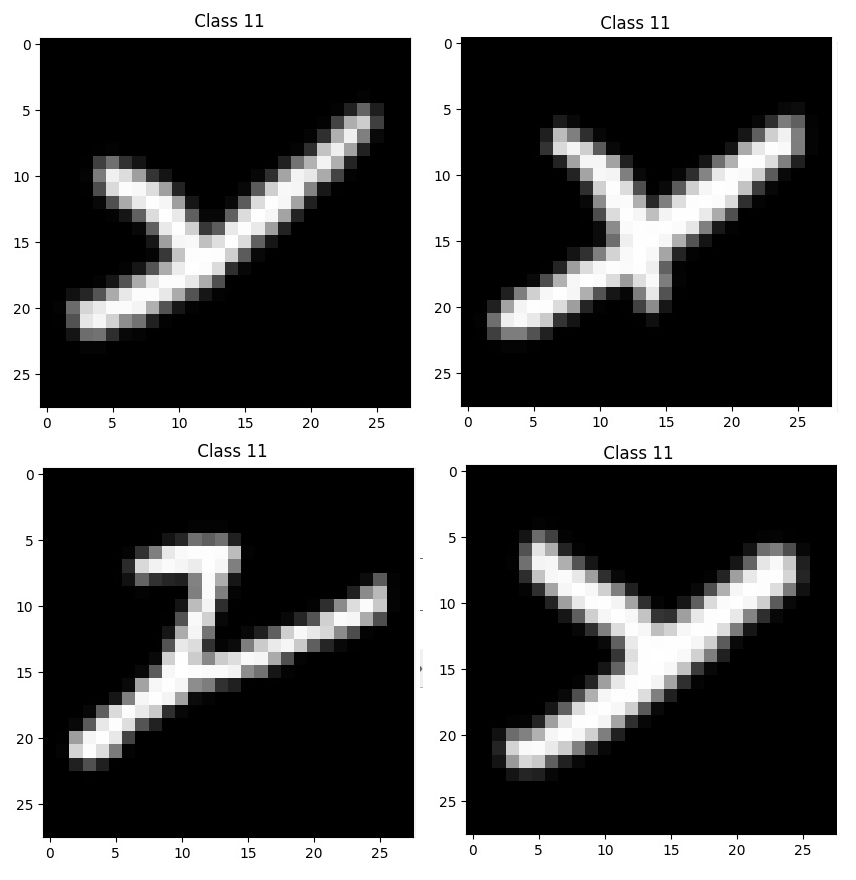
\includegraphics[width=0.35\textwidth]{class11_well.png}}
		\qquad
		\subfloat[]{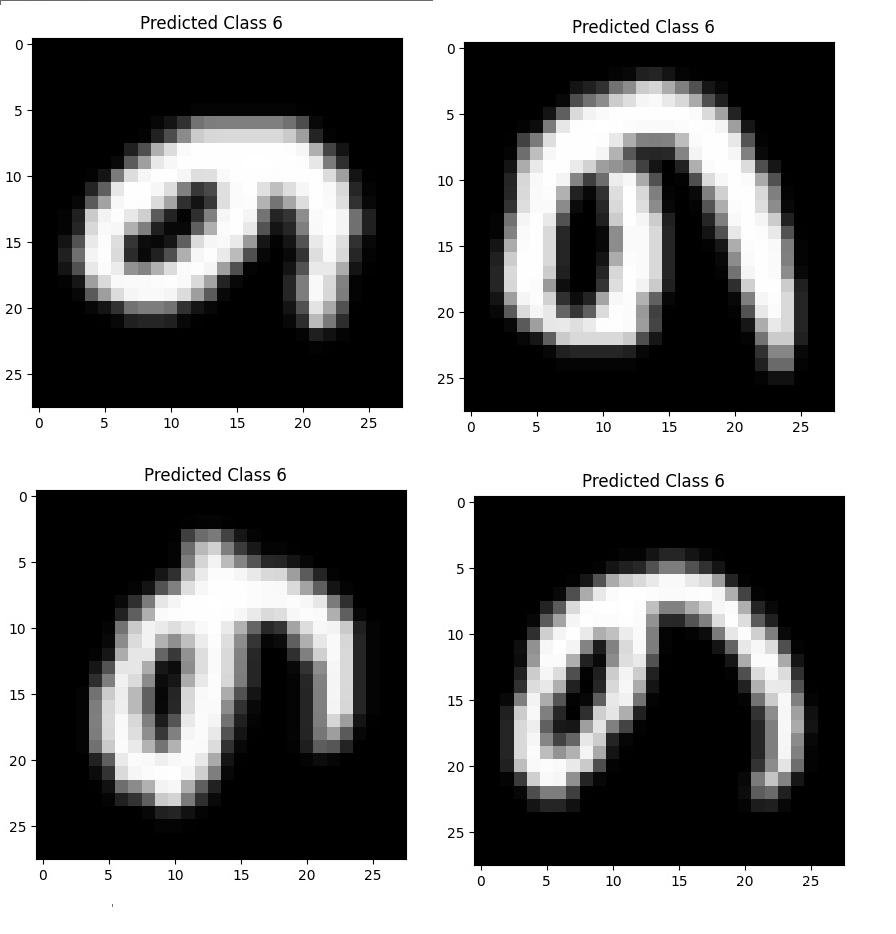
\includegraphics[width=0.35\textwidth]{class6_well.png}}
	}
	\caption[Classes]{Images of class 11 and class 6}
	\label{fig:classes_116}
\end{figure}
We can see that the images of this classes are different from each other and have unique features, this fact helps for better prediction.


%\bibliographystyle{plain}
%\bibliography{bibliography.bib}
\end{document}